\chapter{USE OF RATES AND DIFFERENTIALS IN SOLVING PROBLEMS}

\section{Introductory Remarks}
In the preceding chapter we have worked out a number of examples illustrating the use of the differential formulas. In those illustrations and the corresponding exercises for the reader, the functions or algebraic expressions were given already formed. In applying the principles of rates and differentials to problems which are simply described without being formulated, however, the function must first be formulated mathematically.

In the present chapter we give the detailed solutions of a number of such problems showing the use and application of rates and differentials in cases in which variable quantities are involved. In these solutions the formulation of one variable as a function of another is shown in full and the differentiation is carried out by the appropriate formula in each case. The formula is not designated by letter as in the preceding chapter, however, and the reader is advised to look up the proper formula and follow out its application step by step in each case. The differentiations used involve only the algebraic formulas so far derived.

In each case the results obtained are interpreted when their significance is not immediately obvious.

\section{Illustrative Problems}
\subsection*{Problem 1}
A man walks directly across a street at the rate of five feet per second and his path passes four feet from a lamp post on the opposite side from which he started. The lamp throws his shadow on a wall along the side of the street from which he started. If the lamp is thirty-six feet from the wall, how fast is the shadow moving when the man is sixteen feet from the wall? When he is twenty-six feet away? Where is the man when his shadow moves at the same rate at which he is walking?

\subsection*{Solution}
Let AS represent the wall, BL the opposite side of the street, AB the path of the man, L the position of the lamp, P the position of the man and S that of his shadow at any moment, as shown in Fig.\ref{fig:shadow}. Then AB = 36 feet, BL = 4 feet, and if we let AP = $x$ represent the distance of the man from the wall at any instant, then the rate at which he is walking is $dx/dt = 5$ ft./sec. If we let AS = $y$ represent the distance of the shadow from the starting point at the same instant, the speed of the shadow is the rate at which $y$ is increasing. That is, we have to find $dy/dt$.

\begin{figure}[h]
\centering
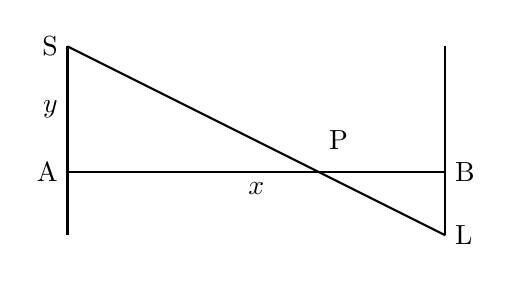
\begin{tikzpicture}[scale=0.8]
    % Draw the vertical walls
    \draw[thick] (0,3) -- (0,0);
    \draw[thick] (6,3) -- (6,0);
    
    % Add S label
    \node[left] at (0,3) {S};
    
    % Draw the horizontal line (man's path) with A and B labels
    \draw[thick] (0,1) -- (6,1) node[midway, below] {$x$};
    \node[left] at (0,1) {A};
    \node[right] at (6,1) {B};
    
    % Draw the straight diagonal line from S to L
    \draw[thick] (0,3) -- (6,0);
    
    % Add L label
    \node[right] at (6,0) {L};
    
    % Add point P label further right and up from intersection
    \node[above right] at (4,1.2) {P};
    
    % Add y label
    \node[left] at (0,2) {$y$};

\end{tikzpicture}
\caption{Man walking across street with shadow cast by lamp post.}
\label{fig:shadow}
\end{figure}

In order to find $dy/dt$ we must first find the relation between the man's distance $x$ and that of the shadow, $y$, that is, express $y$ as a function of $x$.

In order to do this we make use of the relations between the various distances given by the figure.

Since AS and BL are parallel and AB is perpendicular to both, the triangles APS and BPL are right triangles, and since the vertical angles at P are equal, the two triangles are similar and, therefore, the corresponding sides are proportional. That is,

\[AS : AP :: BL : BP\]

Using the values given above for AS, AP and BL and noticing that BP = AB - AP = 36 - x, this proportion becomes

\[y : x :: 4 : (36-x)\]

Solving for $y$,
\[y = \frac{4x}{36-x}\]
and this is the desired relation between $y$ and $x$.

We must now find the differential $dy$, and since $y$ equals the fraction on the right side of the equation the differential of $y$ equals the differential of this fraction. Therefore,
\[dy = \frac{(36-x)\cdot d(4x) - 4x\cdot d(36-x)}{(36-x)^2}\]

and next performing the indicated differentiations in the numerator of the last expression it becomes
\[dy = \frac{(36-x)\cdot 4\,dx - 4x\cdot(-dx)}{(36-x)^2} = \frac{144\,dx}{(36-x)^2}\]

Hence,
\[\frac{dy}{dt} = \frac{144}{(36-x)^2}\cdot\frac{dx}{dt}\]

But $dx/dt = 5$, therefore,
\[\frac{dy}{dt} = \frac{720}{(36-x)^2} \tag{a}\]

which gives the rate at which the shadow is moving when the man is at any distance $x$ from the wall.

When $x = 16$, $\frac{dy}{dt} = \frac{720}{(36-16)^2} = 18$ ft./sec.

When $x = 26$, $\frac{dy}{dt} = \frac{720}{(36-26)^2} = 7.2$ ft./sec.

When $\frac{dy}{dt} = \frac{dx}{dt}$, then we have the same factor on both sides in equation (a) above and cancelling this factor gives
\[1 = \frac{144}{(36-x)^2}\]

as the condition, and from this the value of $x$ is to be determined in order to find the position of the man. Taking the square root of both sides of the last expression we get
\[36-x = \pm 12, \text{ and } x = 36 \pm 12 = 24 \text{ or } 48 \text{ feet}\]

Since the street is only 36 feet wide the 48 is an impossible result and therefore the man is at a distance 24 feet from the wall when his shadow moves at the rate at which he is walking. This is only true for an instant, however; immediately before that time the shadow is moving more slowly and immediately afterwards it is moving more rapidly, as indicated by the rates of the shadow found above when the man is 16 feet and 26 feet from the wall.

The phenomenon considered in this problem has been noticed by everyone, but the problem is not easily solved without the calculus method of rates.

\subsection*{Problem 2}
The top of a ladder 20 ft. long is resting against a vertical wall on a level pavement when the ladder begins to slide downward and outward. At the moment when the foot of the ladder is 12 feet from the wall it is sliding away from the wall at the rate of two feet per second. How fast is the top sliding downward at that instant? How far is the foot of the ladder from the wall when it and the top are moving at the same rate?

\subsection*{Solution}
In Fig.\ref{fig:ladder} let OA represent the pavement, OB the wall, and AB the ladder; the arrows represent the direction of motion. Let $x$ represent the distance OA of the foot of the ladder from the wall, and $y$ the distance OB of the top from the pavement. We have then from the statement of the problem AB = 20 feet, $dx/dt = 2$ ft./sec., and we are to find $dy/dt$ and also find when $dy/dt = dx/dt$.

\begin{figure}[h]
\centering
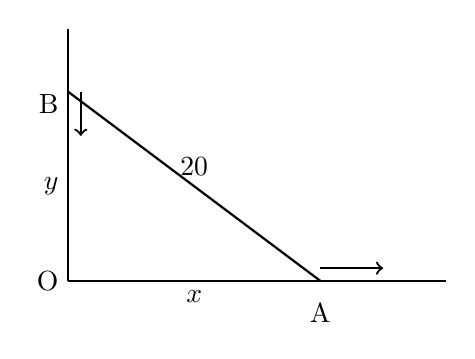
\begin{tikzpicture}[scale=0.8]
    % Draw the ground
    \draw[thick] (0,0) -- (6,0);
    
    % Draw the wall
    \draw[thick] (0,0) -- (0,4);
    
    % Add labels
    \node[left] at (0,0) {O};
    \node[below] at (4,-0.2) {A};
    \node[left] at (0,2.8) {B};     % Adjusted B label position
    
    % Draw the ladder (20 units long)
    \draw[thick] (0,3) -- (4,0) node[midway, above] {20};
    
    % Add y label
    \node[left] at (0,1.5) {$y$};
    
    % Add x label
    \node[below] at (2,0) {$x$};
    
    % Add arrows showing motion
    \draw[->, thick] (4,0.2) -- (5,0.2);  % Horizontal arrow at bottom
    \draw[->, thick] (0.2,3) -- (0.2,2.3);  % Vertical arrow at top
    
\end{tikzpicture}
\caption{Ladder sliding down wall with motion vectors.}
\label{fig:ladder}
\end{figure}

First we must express $y$ in terms of $x$. This is done from the figure by noting that since OA is horizontal and OB is vertical the triangle AOB is a right triangle. Therefore,
\[OB^2 + OA^2 = AB^2\]
that is,
\[y^2 + x^2 = 20^2 = 400\]

Therefore,
\[y = \sqrt{400-x^2}\]
is the desired relation between $y$ and $x$, that is, the expression of $y$ as a function of $x$. In order to get the rate $dy/dt$, we must from this equation find $dy$ and then divide by $dt$.

Differentiating the equation by the square root formula,
\[dy = d(\sqrt{400-x^2}) = \frac{d(400-x^2)}{2\sqrt{400-x^2}} = \frac{-d(x^2)}{2\sqrt{400-x^2}}\]
\[= \frac{-2x\,dx}{2\sqrt{400-x^2}} = -\frac{x\,dx}{\sqrt{400-x^2}}\]

Therefore,
\[\frac{dy}{dt} = -\frac{x}{\sqrt{400-x^2}}\cdot\frac{dx}{dt} \tag{a}\]

Now we had given $dx/dt = 2$ and are to find $dy/dt$ when the distance $x = 12$. Putting these values in the result (a), we get
\[\frac{dy}{dt} = -\frac{12}{\sqrt{400-144}}\cdot 2 = -\frac{24}{\sqrt{256}} = -\frac{24}{16} = -1.5\text{ ft./sec.}\]

The negative sign of $dy/dt$ indicates that $y$ is decreasing, that is, the top of the ladder is moving downward.

To find when $dy/dt = dx/dt$, put $dy/dt$ for $dx/dt$ in formula (a). Then the factor $dy/dt$ cancels on each side, and we have
\[1 = -\frac{x}{\sqrt{400-x^2}}\]

Hence,
\[\sqrt{400-x^2} = -x\]
\[400-x^2 = x^2\]
\[400 = 2x^2\]
\[x^2 = 200\]
\[x = \sqrt{200} = 14.14\text{ ft.}\]

That is, at the instant when the foot of the ladder is 14.14 feet from the wall the foot and top are moving at the same rate.

\subsection*{Problem 3}
A stone is dropped into a quiet pond and waves move in circles outward from the place where it strikes, at a speed of three inches per second. At the instant when the radius of one of the wave rings is three feet, how fast is its enclosed area increasing?

\subsection*{Solution}
Let $R$ be the radius and $A$ the area of one of the circular waves. Then $A = \pi R^2$ and $dA = d(\pi R^2) = 2\pi R\,dR$.

The speed of the wave outward from the center is the rate at which the radius increases, $dR/dt$. Hence, $dR/dt = 3$ in./sec. = $\frac{1}{4}$ ft./sec., and at the instant when the radius is $R = 3$ feet the area is increasing at the rate
\[\frac{dA}{dt} = 2\pi R\cdot\frac{dR}{dt} = 2\pi\cdot 3\cdot\frac{1}{4} = \frac{3\pi}{2} \approx 4.71\text{ sq. ft./sec.}\]

\begin{figure}[h]
    \centering
    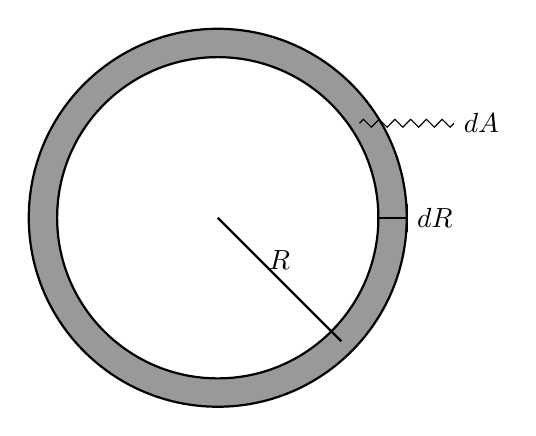
\begin{tikzpicture}[scale=1.2]
        % Draw outer and inner circles with filled ring
        \fill[black!40] (0,0) circle (2);
        \fill[white] (0,0) circle (1.7);
        \draw[thick] (0,0) circle (2);
        \draw[thick] (0,0) circle (1.7);
        
        % Add radius line and label rotated 45 degrees downward
        \draw[thick] (0,0) -- ({1.85/sqrt(2)},{-1.85/sqrt(2)}) node[midway, above] {$R$};
        
        % Add strip width label with small vertical lines
        \draw[thick] (2,-0.15) -- (2,0.15);
        \draw[thick] (1.7,-0.15) -- (1.7,0.15);
        \draw[thick] (1.7,0.0) -- (2,0.0)  node[right] {$dR$};
        
        % Add dA label with zigzag arrow pointing to shaded area
        \draw[decorate, decoration={zigzag, segment length=2mm, amplitude=0.5mm}] 
            (1.5,1.0) -- (2.5,1.0) node[right] {$dA$};
        
    \end{tikzpicture}
    \caption{Circular wave expanding in pond with differential area and radius shown.}
    \label{fig:wave}
\end{figure}

This problem can be formulated graphically by means of Fig.\ref{fig:wave}. As the circular wave moves from the inner dotted circle to the very near outer one, the differential of the radius is $dR$ and the corresponding differential increase of area is the shaded ring of area $dA$.

Now the average radius of this ring strip is $R$ and, therefore, its length is $2\pi R$. Its area is the product of length by width:
\[dA = 2\pi R\cdot dR\]
which is the result already obtained by differentiation. From this result, the rate is found as before.

\subsection*{Problem 4}
Water runs into a conical paraffine paper cup five inches high and three inches across the top, at the rate of one cubic inch per second. When it is just half filled how rapidly is the surface of the water rising?

\subsection*{Solution}
Let Fig.\ref{fig:cone} represent the shape and dimensions of the cup. Then, if $v$ represents the volume of water already in the cup when $h$ is the height of the surface above the point of the cone, the rate at which water is running in is the rate of increase of the volume, $dv/dt$, and $dh/dt$ is the rate of increase of the height $h$, that is, the rate at which the surface is rising.

\begin{figure}[h]
    \centering
    \begin{tikzpicture}[scale=1.2]
        % Draw the cone outline
        \draw[thick] (0,0) -- (3,4) -- (-3,4) -- cycle;
        
        % Calculate water level points - adjusted to be proportional
        \coordinate (WL) at (0,1.5);  % water level height
        \coordinate (WLeft) at (-1.125,1.5);  % proportionally smaller than top width
        \coordinate (WRight) at (1.125,1.5);  % proportionally smaller than top width
        
        % Draw and fill water region with pattern
        \fill[pattern=horizontal lines, pattern color=black!40] 
            (0,0) -- (-1.125,1.5) -- (1.125,1.5) -- cycle;
        
        % Draw the water level line
        \draw[thick] (-1.125,1.5) -- (1.125,1.5);
        
        % Add dimension lines and labels
        % Top width D
        \draw[thick,<->] (-3,4.3) -- (3,4.3) node[midway, above] {$D$};
        
        % Water level width d
        \draw[thick,<->] (-1.125,1.8) -- (1.125,1.8) node[midway, above] {$d$};
        
        % Total height H
        \draw[thick,<->] (3.3,0) -- (3.3,4) node[midway, right] {$H$};
        
        % Water height h
        \draw[thick,<->] (-3.3,0) -- (-3.3,1.5) node[midway, left] {$h$};
        
    \end{tikzpicture}
    \caption{Conical cup filling with water, showing dimensions and water level.}
    \label{fig:cone}
\end{figure}

The indicated dimensions $d$ and $h$ (this $d$ has nothing to do with differentiation) are then variables and $D$, $H$ are constants. We have $dv/dt = 1$ cu.\ in.\ per sec.\ and are to find $dh/dt$ at the instant when $h$ is such that the cup is half filled.

The volume of the cone is one third the base area times the altitude. Hence, the total volume is
\[\frac{\pi D^2H}{12} = \frac{\pi(3^2)\cdot 5}{12} = 11.7\text{ cu.\ in.}\]
with the dimensions given. Therefore, when half filled, the volume of the water is $v = 5.85$ cu.\ in. We must, therefore, find $dh/dt$ when $v = 5.85$ and $dv/dt = 1$, and to do this we must have a relation between $h$ and $v$, that is, express $h$ as a function of $v$.

The volume formula in terms of the altitude $h$ furnishes the relation desired. This formula is, as above,
\[v = \frac{\pi d^2h}{12}\]
hence,
\[h d^2 = \frac{12v}{\pi} \tag{a}\]

This formula, however, contains not only the desired variables $h$ and $v$, but also the undesired variable $d$. This variable must, therefore, be expressed in terms of either $h$ or $v$. It is simpler to express $d$ in terms of $h$ by means of the proportionality between $D$, $H$, which are known, and $d$, $h$. In Fig.\ref{fig:cone} the two inverted triangles of bases (diameters) $D$, $d$ and heights $H$, $h$ are similar and therefore $d : h :: D : H$. Therefore,
\[\frac{d}{h} = \frac{D}{H} = \frac{3}{5} = 0.6\]
\[\therefore d = 0.6h, \text{ and } d^2 = 0.36h^2\]

Using this value of $d^2$ in formula (a) above, it becomes
\[h(0.36h^2) = \frac{12v}{\pi}\]
\[0.36h^3 = \frac{12v}{\pi}\]
hence,
\[h^3 = \frac{12v}{0.36\pi}\]

By taking the cube root of the numerical fraction and expressing the cube root of $v$ as the $\frac{1}{3}$ power, we get finally as the desired functional relation between $h$ and $v$,
\[h = 2.20v^{\frac{1}{3}} \tag{b}\]

Differentiating by the power formula,
\[dh = 2.2d(v^{\frac{1}{3}}) = 2.2(\frac{1}{3}v^{-\frac{2}{3}}dv) = \frac{0.74}{v^{\frac{2}{3}}}dv\]

Therefore, when $v = 5.85$ (half filled) and $dv/dt = 1$ (rate of inflow),
\[\frac{dh}{dt} = \frac{0.74}{(5.85)^{\frac{2}{3}}} = \frac{0.74}{\sqrt[3]{34.2}} = 0.23\text{ in./sec.}\]
is the rate at which the surface of the water is rising.

This problem illustrates a condition which is often met in calculus: the algebra and geometry or other calculations which are necessary for the formulation before the calculus can be applied are longer than the direct solution of the calculus problem itself. Thus in this case after $h$ was expressed as a function of $v$ in formula (b) the differentiation and calculation of the rate were simple operations. The tedious part of the solution of the problem consisted not in the application of the calculus, but in deriving the functional relation (b) and in calculating when the cup was half filled.

\subsection*{Problem 5}
A ship is sailing due north at the rate of 20 miles per hour. At a certain time another ship crosses its route 40 miles north sailing due east 15 miles per hour. (i) At what rate are the ships approaching or separating after one hour? (ii) After two hours? (iii) After how long are they momentarily neither approaching nor separating? (iv) At that time, how far apart are they?

\subsection*{Solution}
We must express the distance between the ships as a function of the time after the second crossed the path of the first. The rate of change of this distance is then their speed of approach or separation. In Fig.\ref{fig:ships}, let $P$ represent the position of the first ship when the second crosses its path at $O$, 40 miles due north.

\begin{figure}[h]
    \centering
    \begin{tikzpicture}[scale=1.2]
        % Draw the vertical line with arrow
        \draw[thick, ->] (0,-2) -- (0,4);
        
        % Draw the horizontal line with arrow
        \draw[thick] (0,3) -- (4,3);
        \draw[thick, ->] (4,3) -- (4.5,3);
        
        % Add points
        \node[left] at (0,-1) {$P$};
        \node[left] at (0,3) {$O$};
        \node[above] at (3,3) {$A$};
        \node[left] at (0,1) {$B$};
        
        % Add distance labels
        \node[above] at (1.5,3) {$x$};
        \node[right] at (0,2) {$y$};
        \node[right] at (1.8,2) {$s$};
        
        % Draw the distance line s
        \draw[thick] (0,1) -- (3,3);
        
        % Add movement arrows for ships
        \draw[->, thick] (3.2,3.2) -- (3.7,3.2);  % Ship A moving east
        \draw[->, thick] (-0.2,1.2) -- (-0.2,1.7);  % Ship B moving north
        
    \end{tikzpicture}
    \caption{Two ships moving at right angles, showing their relative positions and motion.}
    \label{fig:ships}
\end{figure}

After a certain time $t$ hours the ship sailing east will have reached a point $A$, and the ship sailing north will have reached a point $B$. The distance between them is then $AB$.

If we take $O$ as reference point, and let $OA = x$, $OB = y$, $AB = s$, then $OP = 40$ and
\[s^2 = x^2 + (y-40)^2 \tag{a}\]

Now, the rate of the ship $B$ is $dy/dt = 20$ and of the ship $A$ $dx/dt = 15$ miles per hour. Therefore, after the time $t$ hours has passed, $B$ has covered the distance $PB = 20t$ and the ship $A$ the distance $OA = 15t$. Then, $OB = OP + PB = 40 + 20t$. Therefore,
\[x = 15t, \quad y = 40 + 20t \tag{b}\]

Using these values of $x$, $y$ in equation (a) gives for the distance
\[s^2 = (15t)^2 + (40 + 20t - 40)^2 = 225t^2 + 400t^2 = 625t^2\]
\[\therefore s = 25t \tag{c}\]

This is the desired relation between the distance between the ships, and the time $t$ after the crossing at $O$. If at any time the rate $ds/dt$ is positive, the distance is increasing, that is, the ships are separating. If at any time it is negative they are approaching. To find the rate $ds/dt$ we must differentiate equation (c). Using the power formula:
\[ds = d(25t) = 25\,dt\]
\[\therefore \frac{ds}{dt} = 25 \tag{d}\]

In order to calculate the required results (i) to (iv) we proceed as follows:

(i) After 1 hour $t = 1$ and $ds/dt = 25$ mi./hr.\ and the ships are separating.

(ii) After 2 hours $t = 2$ and $ds/dt = 25$ mi./hr.\ and they are still separating.

(iii) Since $ds/dt$ is constant and positive, the ships are always separating at the same rate. There is no time when they are neither approaching nor separating.

(iv) After 1 hour, equations (b) give
\[x = 15\text{ mi.}, \quad y = 60\text{ mi.}\]
The distance between the ships is then according to equation (c)
\[s = 25\text{ mi.}\]

This completes the solution. This problem illustrates how the derivative can give us information about the relative motion of objects.

\subsection*{Problem 6}
An aeroplane flying horizontally in a straight line at a rate of 60 miles an hour and an elevation of 1760 feet crosses at right angles a straight level road just as an automobile passes underneath at 30 miles an hour. How far apart are they and at what rate are they separating one minute later?

\subsection*{Solution}
In Fig.\ref{fig:airplane}, let $C$ represent the position of the aeroplane at the instant when the automobile is vertically below it at the point $O$.

\begin{figure}[h]
    \centering
    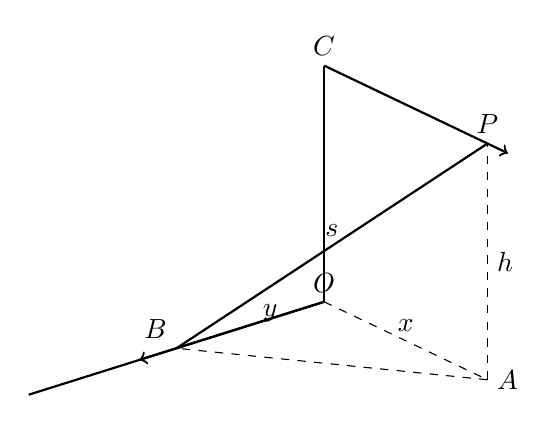
\begin{tikzpicture}[rotate around y=-40] %[x={(1cm,0cm)}, y={(-0.5cm,-0.5cm)}, z={(0cm,1cm)}, rotate around={-15:(0,0,0)}]
        % Draw the vertical line CO
        \draw[thick] (0,3,0) -- (0,0,0);
        \node[above] at (0,3,0) {$C$};
        
        % Draw the horizontal plane with dashed lines
        \draw[dashed] (0,0,0) -- (4,0,0);  % OA
        \draw[dashed] (4,0,0) -- (0,0,2);  % AB
        \draw[thick] (0,0,0) -- (0,0,4);  % OB extension
        
        % Draw the airplane path CP with arrow
        \draw[thick] (0,3,0) -- (4,3,0);
        \draw[->, thick] (4,3,0) -- (4.5,3,0);
        \node[above] at (4,3,0) {$P$};
        
        % Draw the vertical line PA
        \draw[dashed] (4,0,0) -- (4,3,0);
        \node[right] at (4,0,0) {$A$};
        
        % Draw the car path OB with arrow
        \draw[thick] (0,0,0) -- (0,0,2);
        \draw[->, thick] (0,0,2) -- (0,0,2.5);
        \node[above left] at (0,0,2) {$B$};
        \node[above] at (0,0,0) {$O$};
        
        % Draw the distance line PB (s)
        \draw[thick] (4,3,0) -- (0,0,2);
        
        % Add labels
        \node[above] at (2,0,0) {$x$};
        \node[left] at (0,0,0.5) {$y$};
        \node[right] at (4,1.5,0) {$h$};
        \node[above] at (2,1.5,1) {$s$};
        
    \end{tikzpicture}
    \caption{Airplane and automobile moving in perpendicular directions, showing their relative positions and motion.}
    \label{fig:airplane}
\end{figure}

Then $CP$ is the direction of the aeroplane and $OB$ that of the automobile. If the arrows indicate the motion, then after a time $t$ minutes they will occupy the positions $P$ and $B$ and the straight line distance between them is the inclined diagonal $PB = s$. We have to find an expression for $s$ at any time $t$ and also its rate $ds/dt$.

Draw $OA$ parallel to $CP$; draw the vertical line $PA$ to the point vertically under $P$; draw $AB$; and denote the distances by $x$, $y$, $h$ as shown. Then $OAB$ is a right triangle with legs $x$ and $y$ and hypotenuse $AB$, and $PAB$ is a right triangle with legs $AP$ and $AB$ and hypotenuse $PB = s$. Therefore,
\[s^2 = AB^2 + h^2, \text{ and } AB^2 = x^2 + y^2\]
\[\therefore s^2 = x^2 + y^2 + h^2 \tag{a}\]

Since the aeroplane is travelling at the rate $dx/dt = 60$ miles per hour $= 1$ mi./min.\ and the automobile at the rate $dy/dt = 30$ miles per hour $= \frac{1}{2}$ mi./min., then, at the end of $t$ minutes they are at the distances from the crossing point of
\[CP = x = t, \quad OB = y = \frac{1}{2}t, \quad OC = h = \frac{1}{3}\text{ miles}\]
since 1760 feet is one third of a mile. Using these values of $x$, $y$, $h$ in (a) we have
\[s^2 = t^2 + \frac{1}{4}t^2 + \frac{1}{9} = \frac{5}{4}t^2 + \frac{1}{9}\]
\[\therefore s = \sqrt{\frac{5}{4}t^2 + \frac{1}{9}} \tag{b}\]
is the distance between the aeroplane and the automobile at any time $t$ minutes after the crossing, and the rate at which they are separating is $ds/dt$. From (b)
\[ds = d\left(\sqrt{\frac{5}{4}t^2 + \frac{1}{9}}\right) = \frac{d(\frac{5}{4}t^2 + \frac{1}{9})}{2\sqrt{\frac{5}{4}t^2 + \frac{1}{9}}} = \frac{\frac{5}{2}t\,dt}{\sqrt{\frac{5}{4}t^2 + \frac{1}{9}}}\]
\[\therefore \frac{ds}{dt} = \frac{\frac{5}{2}t}{\sqrt{\frac{5}{4}t^2 + \frac{1}{9}}} \tag{c}\]
is the rate at which they are separating at the time $t$.

Using (b) and (c) we are to calculate the distance and the rate $ds/dt$ at the end of one minute. Thus $t = 1$ and by (b)
\[s = \sqrt{\frac{5}{4} + \frac{1}{9}} = \sqrt{\frac{45}{36} + \frac{4}{36}} = \sqrt{\frac{49}{36}} = \frac{7}{6}\text{ miles}\]
by (c),
\[\frac{ds}{dt} = \frac{\frac{5}{2}}{\sqrt{\frac{49}{36}}} = \frac{\frac{5}{2}}{\frac{7}{6}} = \frac{15}{7}\text{ mi./min.}\]

In the same way formulas (b) and (c) will give the distance and relative velocity of the two at any other time in minutes.

\section*{Exercises}
\addcontentsline{toc}{subsection}{Exercises}

\begin{enumerate}
    \item Air is blown into a spherical rubber balloon at such a rate that the radius is increasing at the rate of one-tenth inch per second. At what rate is the air being blown in when the radius is two inches? 
    
    (Hint: The required rate is $dV/dt$, where $V$ is the volume.)

    \item A metal plate in the shape of an equilateral triangle is being heated in such a way that each of the sides is increasing at the rate of ten inches per hour. How rapidly is the area increasing at the instant when each side is 69.28 inches?

    \item Two points move, one on the $OX$ axis and one on $OY$, in such a manner that in $t$ minutes their distances from $O$ are
    \[x = 2t - 6t, \quad y = 6t - 9\]
    feet.
    \begin{enumerate}
        \item[(a)] At what rate are they approaching or separating after one minute?
        \item[(b)] After three minutes?
        \item[(c)] When will they be nearest together?
    \end{enumerate}
    (Hint: Find $s$ and $ds/dt$. In (c) put $ds/dt = 0$.)

    \item A man whose height is six feet walks directly away from a lamp post at the rate of three miles an hour on a level pavement. If the lamp is ten feet above the pavement, at what rate is the end of his shadow travelling?
    
    (Suggestion: Draw a figure and denote the variable distance of the man from the post by $x$, that of the end of the shadow by $y$, and express $y$ as a function of $x$ by similar triangles.)

    \item At what rate does the shadow in Problem 4 increase in length?

    \item A man is walking along the straight bank of a river 120 feet wide toward a boat at the bank, at a rate of five feet a second. At the moment when he is still fifty feet from the boat how rapidly is he approaching the point on the opposite bank directly across from the boat?
    
    (Draw figure, let $x$ = distance to boat, and formulate distance to point opposite.)

    \item A man standing on a wharf is hauling in a rope attached to a boat, at the rate of four feet a second. If his hands are nine feet above the point of attachment how fast is the boat approaching the wharf when it is twelve feet away?

    \item One end of a wire wound on a reel is fastened to the top of a pole 35 feet high; two men holding the reel on a rod on their shoulders five feet above the level ground walk away from the pole at the rate of five miles an hour, keeping the wire straight. How far are they from the pole when the wire is unwinding at the rate of one mile an hour?

    \item A three-mile wind blowing on a level is carrying a kite directly away from a boy. How high is the kite when it is directly over a point 100 feet away and he is paying out the string at the rate of 88 feet a minute?

    \item Two automobiles are moving along straight level roads which cross at an angle of sixty degrees, one approaching the crossing at 25 miles an hour and the other leaving it at 30 miles an hour on the same side. How fast are they approaching or separating from each other at the moment when each is ten miles from the crossing?

    \item Assuming the volume of a tree to be proportional to the cube of its diameter ($V = k\cdot D^3$ where $k$ is a constant) and that the diameter increases always at the same rate, how much more rapidly is the tree growing in volume when the diameter is three feet than when it is six inches?

    \item In being heated up to the melting point, a brick-shaped ingot of silver expands the thousandth part of each of its three dimensions for each degree temperature increase. At what rate per degree ($dV/dT$, where $T$ is the temperature) is its volume increasing when the dimensions are $2 \times 3 \times 6$ inches?

    \item Sand is being poured from a dumping truck and forms a conical pile with its height equal to one third the base diameter. If the truck is emptying at the rate of 720 cubic feet a minute and the outlet is five feet above the ground, how fast is the pile rising as it reaches the outlet?

    \item A block of building stone is to be lifted by a rope 50 ft.\ long passing over a pulley on a window ledge 25 feet above the level ground. A man takes hold of the loose end of the rope which is held five feet above the ground and walks away from the block at ten feet a second. How rapidly will the block begin to rise?

    \item The volume of a sphere is increasing at the rate of 16 cu.\ in.\ per second. At the instant when the radius is 6 in.\ how fast is it increasing?

    \item A rope 28 feet long is attached to a block on level ground and runs over a pulley 12 feet above the ground. The rope is stretched taut and the free end is drawn directly away from the block and pulley at the rate of 13 ft.\ per sec. How fast will the block be moving when it is 5 feet away from the point directly below the pulley?

    \item A tank is in the form of a cone with the point downward, and the height and diameter are each 10 feet. How fast is the water pouring in at the moment when it is 5 feet deep and the surface is rising at the rate of 4 feet per minute?

    \item The hypotenuse $AB$ of a right triangle $ABC$ remains 5 inches long while the other two sides change, the side $AC$ increasing at the rate of 2 in.\ per min. At what rate is the area of the triangle changing when $AC$ is just 3 inches?

    \item A spherical barrage balloon is being inflated so that the volume increases uniformly at the rate of 40 cu.\ ft.\ per min. How fast is the surface area increasing at the moment when the radius is 8 feet?

    \item A fighter plane is flying in a straight line on a level course to cross the course of a bomber which is also flying on a level course in a straight line. The fighter is at a level 500 feet above the bomber, and their courses cross at an angle of 60 degrees. Both planes are headed toward the crossing of their courses and on the same side of it, the bomber flying at 200 miles per hour and the fighter at 300. At the moment when the fighter is 10 miles and the bomber 7 miles from the crossing point, how rapidly are they approaching one another in a straight line joining the two planes?
\end{enumerate}
